\section{Implementation}
In this section, we describe the implementation phase of the project. The project was implemented using Python 2.7.13 with the usage of library SciPy\cite{scipy} for linear data interpolation. All code was tested and evaluated on the Merlin server at FIT BUT.

\label{sec:implementation}

\subsection{Data Acquisition}
\label{sec:data-filter}
First, job data were queried and filtered according to several rules:
\begin{itemize}
    \setlength\itemsep{0em}
    \item job runtime must be between 10 and 60 minutes
    \item job must occupy the whole node (multiplies of 16 cores)
    \item job must be run in 21-day period (30. 10. 2017 -- 21. 11. 2017)
\end{itemize}

These rules were satisfied by 442 jobs in total with their runtime closer to 10 minutes than 60 minutes. The Examon framework was run only on a small portion of Galileo cluster and therefore not all filtered jobs had metric data present in the metric database.

%\begin{figure}[ht]
%    \centering
%    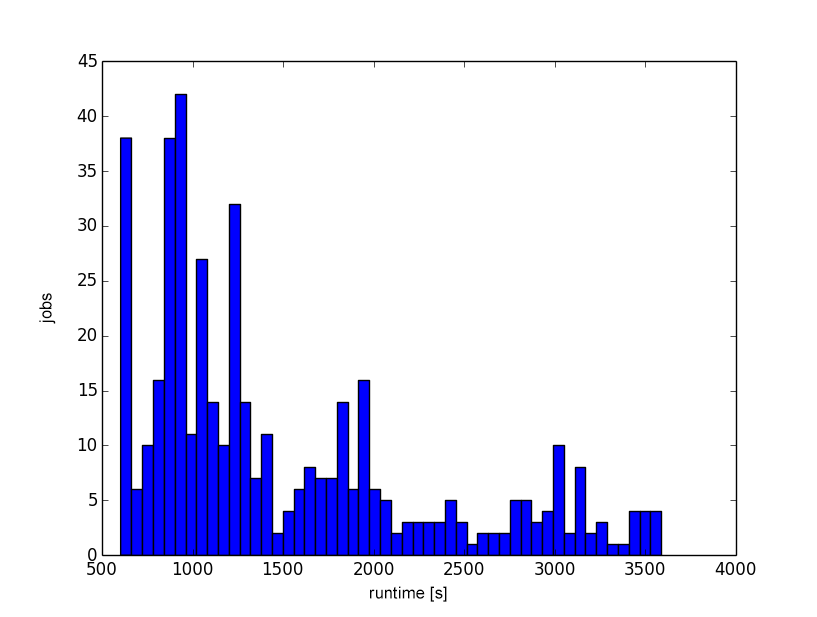
\includegraphics[width=0.5\linewidth]{histogram}
%    \caption{Histogram of jobs' runtimes}
%    \label{fig:histogram}
%\end{figure}

This resulted in 32 jobs which gave enough diversity for correct classification. All data points were aggregated by 30 seconds on cluster level\footnote{Averaging every used core and node in the job to one time serie per metric.} using averaging aggregator available in KairosDB. There are 19 jobs classified as suspicious and 120 out of 384 metric data vectors classified as suspicious.

The rule of minimum 10 minutes is because of any shorter job is usually a development, not the production version of a program and in current HPC facilities, such program is very cheap to run and therefore no deep performance analysis is needed. The same goes for jobs smaller than one node (16~cores in case of Galileo supercomputer).

Jobs longer than one hour are not suited for training the network because of too large input vectors exceeding the scope of this project and the loss of information in further data processing.

\subsection{Data Labelling}
In order to correctly label all chosen jobs and their metrics, a simple graphical user interface was made. The GUI is based on Examon Web which is an extension of Examon framework visualizing specific views of all collected data.

Visualization is done in time series fashion using Dygraphs library. This helps to better understand the in time correlations between all metrics combined.

The GUI is shown in figure \ref{fig:ex-labeler} where you can see a checkbox for each metric and at the bottom a checkbox for the whole job. The metric checkbox labels the accompanying metric of suspicious behaviour and job one of suspicious behaviour of the job as a whole. A suspicious metric or job is labelled with value $1.0$ and unsuspicious was labelled by value $0.0$.

\begin{figure}[ht]
    \centering
    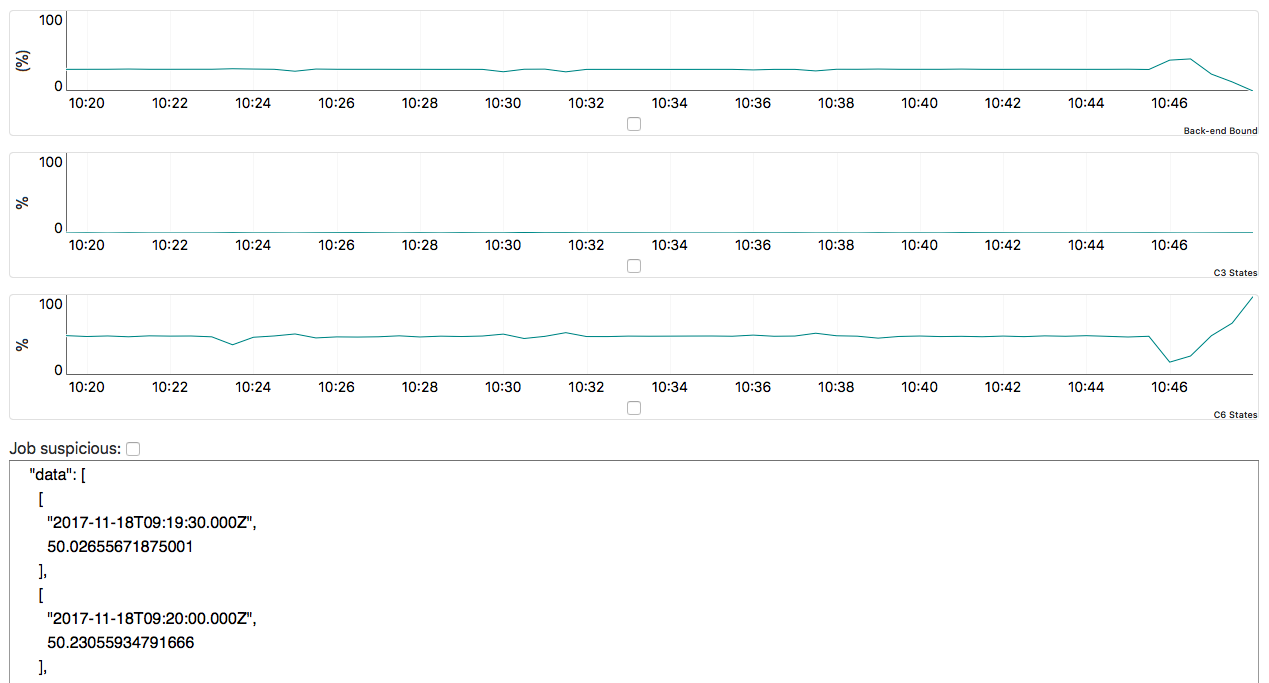
\includegraphics[width=0.65\linewidth]{examon-labeler}
    \caption{Part of Examon Web based data labelling tool}
    \label{fig:ex-labeler}
\end{figure}

\subsection{Data Processing}

After labelling the job all metric data with labels are generated and can be worked on further. All metric vectors were interpolated to 80 values which provide good performance/detail compromise. Larger input vectors resulted in extremely long runs and smaller input vectors resulted in poor outputs of the network.

All values were also normalized to values between $<0.0, 1.0>$.

\subsection{Metric Networks}

To achieve best results/speed combination a backpropagation neural network was created for each metric. This gives us the total of twelve networks completely independent of each other meaning the training process can be fully parallelized.

All metric networks were configured the same way to achieve uniform results. The input layer disposes of 80 neurons with hidden layers of 4 and then 3 neurons and one output neuron.

This configuration was chosen based on trial and error experiments.

\subsection{Job Network}
Once all metric networks compute their output we have a vector of 12 values serving as an input to the job classification network.

The network is created with 12 input neurons, one hidden layer of 4 neurons and one output neuron.

All networks were set to train a maximum of 50 000 epochs or until the sum error reached $0.1$. They were presented with 27 jobs keeping the other 5 jobs as the evaluation dataset. All outputs are a single value--metric networks because of further processing in the job network and the job network because of clearer interpretation of results.
